% pdflatex nn-times-cpu.tex && rm *.aux *.log
% pdftoppm nn-times-cpu.pdf -rx 500 -ry 500 nn-times-cpu -png

\documentclass[varwidth]{standalone}
\usepackage{pgfplots}
\usepackage{graphicx}
\begin{document}

\resizebox{0.95\columnwidth}{!} {
% BIRD
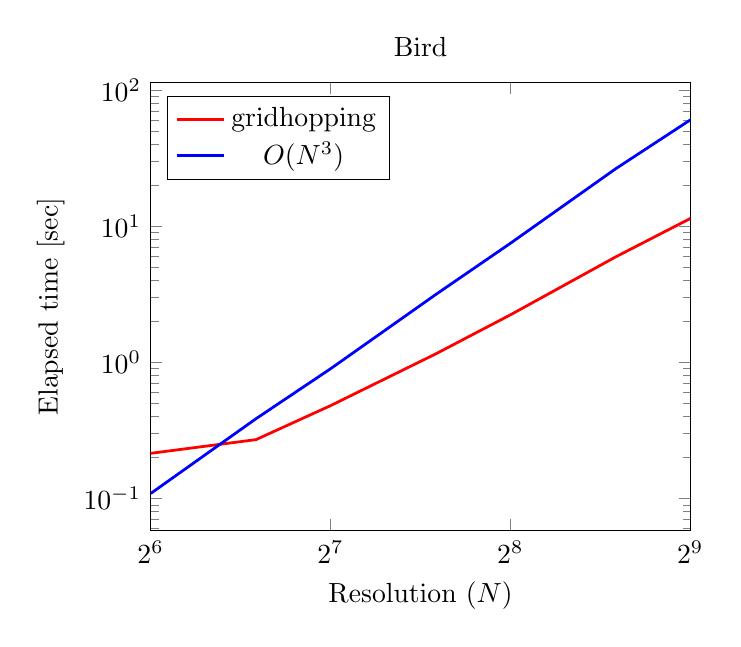
\begin{tikzpicture}
\begin{axis} [
	title=Bird,
	ymode=log,
	xlabel={Resolution ($N$)},
	ylabel={Elapsed time [sec]},
	xmin=64, xmax=512,
	xmode=log, log basis x=2,
	legend pos=north west
]
		\addplot[color=red, line width=1]
			coordinates {
				(64.000000, 0.215000)(96.000000, 0.271000)(128.000000, 0.482000)(192.000000, 1.157000)(256.000000, 2.241000)(384.000000, 5.969000)(512.000000, 11.437000)
			};
		\addplot[color=blue, line width=1]
			coordinates {
				(64.000000, 0.109000)(96.000000, 0.386000)(128.000000, 0.900000)(192.000000, 3.160000)(256.000000, 7.523000)(384.000000, 26.518000)(512.000000, 60.646000)
			};
		\legend{gridhopping,$O(N^3)$}
\end{axis}
\end{tikzpicture}
% FROG
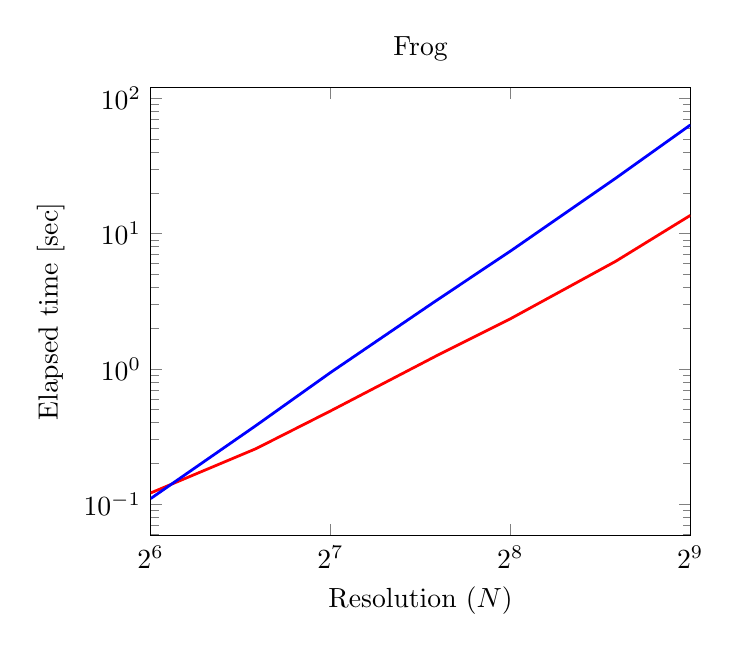
\begin{tikzpicture}
\begin{axis} [
	title=Frog,
	ymode=log,
	xlabel={Resolution ($N$)},
	ylabel={Elapsed time [sec]},
	xmin=64, xmax=512,
	xmode=log, log basis x=2,
	legend pos=north west
]
		\addplot[color=red, line width=1]
			coordinates {
				(64.000000, 0.121000)(96.000000, 0.257000)(128.000000, 0.489000)(192.000000, 1.242000)(256.000000, 2.348000)(384.000000, 6.241000)(512.000000, 13.644000)
			};
		\addplot[color=blue, line width=1]
			coordinates {
				(64.000000, 0.110000)(96.000000, 0.381000)(128.000000, 0.941000)(192.000000, 3.181000)(256.000000, 7.432000)(384.000000, 25.675000)(512.000000, 63.580000)
			};
\end{axis}
\end{tikzpicture}
% CATS
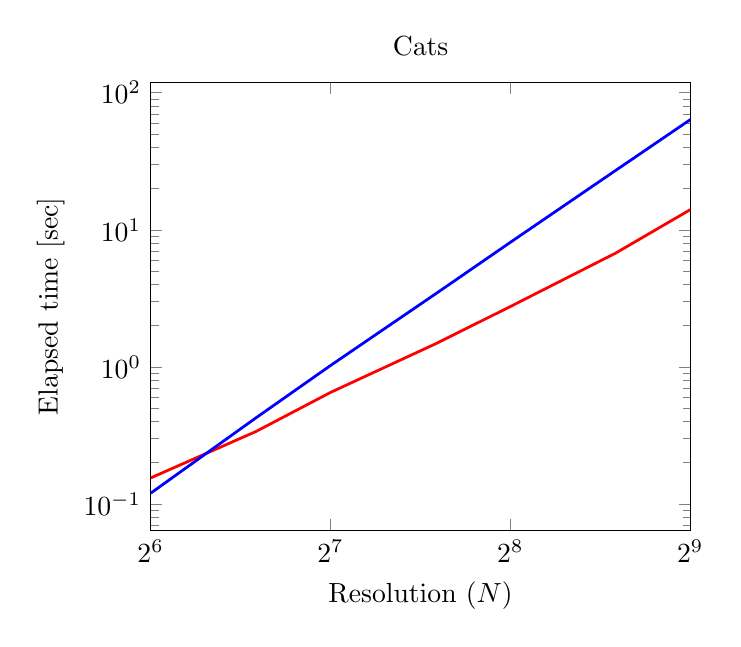
\begin{tikzpicture}
\begin{axis} [
	title=Cats,
	ymode=log,
	xlabel={Resolution ($N$)},
	ylabel={Elapsed time [sec]},
	xmin=64, xmax=512,
	xmode=log, log basis x=2,
	legend pos=north west
]
		\addplot[color=red, line width=1]
			coordinates {
				(64.000000, 0.155000)(96.000000, 0.338000)(128.000000, 0.652000)(192.000000, 1.477000)(256.000000, 2.759000)(384.000000, 6.764000)(512.000000, 14.040000)
			};
		\addplot[color=blue, line width=1]
			coordinates {
				(64.000000, 0.120000)(96.000000, 0.425000)(128.000000, 1.025000)(192.000000, 3.420000)(256.000000, 8.117000)(384.000000, 27.117000)(512.000000, 63.694000)
			};
\end{axis}
\end{tikzpicture}
}
\\
\resizebox{0.95\columnwidth}{!} {
% BUNNY
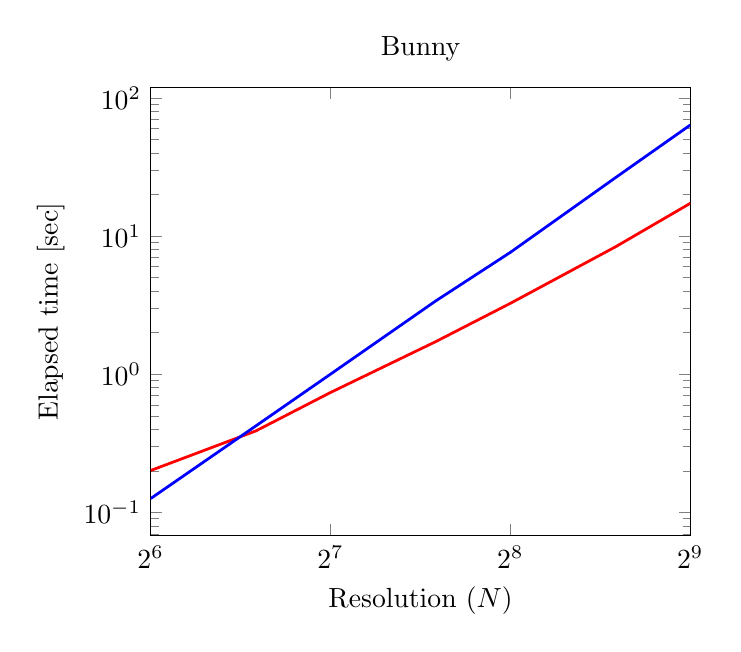
\begin{tikzpicture}
\begin{axis} [
	title=Bunny,
	ymode=log,
	xlabel={Resolution ($N$)},
	ylabel={Elapsed time [sec]},
	xmin=64, xmax=512,
	xmode=log, log basis x=2,
	legend pos=north west
]
		\addplot[color=red, line width=1]
			coordinates {
				(64.000000, 0.201000)(96.000000, 0.389000)(128.000000, 0.738000)(192.000000, 1.722000)(256.000000, 3.261000)(384.000000, 8.366000)(512.000000, 17.258000)
			};
		\addplot[color=blue, line width=1]
			coordinates {
				(64.000000, 0.126000)(96.000000, 0.423000)(128.000000, 1.002000)(192.000000, 3.393000)(256.000000, 7.629000)(384.000000, 26.501000)(512.000000, 63.645000)
			};
\end{axis}
\end{tikzpicture}
% MUSHROOMS
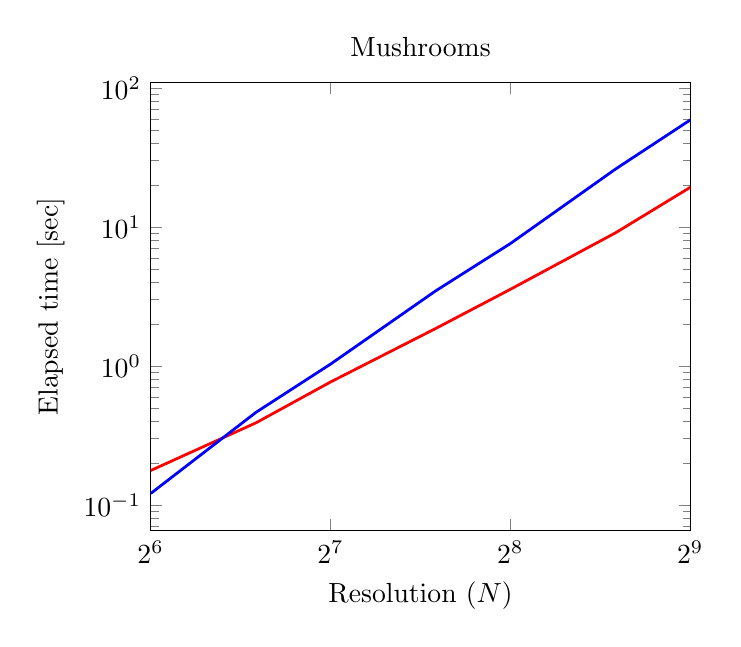
\begin{tikzpicture}
\begin{axis} [
	title=Mushrooms,
	ymode=log,
	xlabel={Resolution ($N$)},
	ylabel={Elapsed time [sec]},
	xmin=64, xmax=512,
	xmode=log, log basis x=2,
	legend pos=north west
]
		\addplot[color=red, line width=1]
			coordinates {
				(64.000000, 0.177000)(96.000000, 0.390000)(128.000000, 0.768000)(192.000000, 1.864000)(256.000000, 3.567000)(384.000000, 9.102000)(512.000000, 19.336000)
			};
		\addplot[color=blue, line width=1]
			coordinates {
				(64.000000, 0.121000)(96.000000, 0.464000)(128.000000, 1.033000)(192.000000, 3.478000)(256.000000, 7.617000)(384.000000, 26.181000)(512.000000, 59.055000)
			};
\end{axis}
\end{tikzpicture}
% WHALE
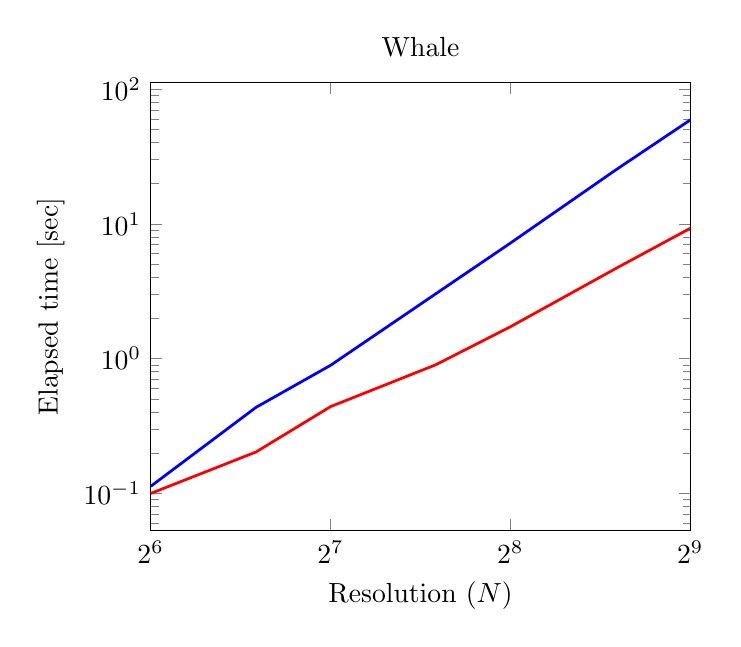
\begin{tikzpicture}
\begin{axis} [
	title=Whale,
	ymode=log,
	xlabel={Resolution ($N$)},
	ylabel={Elapsed time [sec]},
	xmin=64, xmax=512,
	xmode=log, log basis x=2,
	legend pos=north west
]
		\addplot[color=red, line width=1]
			coordinates {
				(64.000000, 0.100000)(96.000000, 0.203000)(128.000000, 0.441000)(192.000000, 0.901000)(256.000000, 1.726000)(384.000000, 4.660000)(512.000000, 9.272000)
			};
		\addplot[color=blue, line width=1]
			coordinates {
				(64.000000, 0.113000)(96.000000, 0.435000)(128.000000, 0.893000)(192.000000, 3.030000)(256.000000, 7.206000)(384.000000, 25.092000)(512.000000, 59.058000)
			};
\end{axis}
\end{tikzpicture}
}

\end{document}
